%Dokumentklasse

%draft als optionohne bilder für bessere performance
%\documentclass[a4paper,12pt,draft]{scrreprt}

%normal mit Bildern
\documentclass[a4paper,12pt]{scrreprt}

\usepackage[left= 3cm,right = 3cm, bottom = 3cm,top = 3cm]{geometry}
%\usepackage[onehalfspacing]{setspace}

% ============= Packages =============
% Dokumentinformationen
\usepackage[
pdftitle={Praktikum - Umwelttechnik},
pdfsubject={},
pdfauthor={Roman-Luca Zank},
pdfkeywords={},	
%Links nicht einrahmen
hidelinks
]{hyperref}

%nur Text zum prüfen des Umfangs

% Standard Packages
%\usepackage[bottom]{footmisc}
\usepackage[utf8]{inputenc}
\usepackage[ngerman]{babel}

\usepackage[T1]{fontenc}
%\usepackage{helvet}

%\renewcommand{\familydefault}{\sfdefault}

\usepackage{graphicx}
\graphicspath{{img/}}
\usepackage{mhchem}
\usepackage{fancyhdr}
\usepackage{lmodern}
\usepackage{color}
\usepackage{placeins}
\usepackage{booktabs}
\usepackage{caption}
\usepackage[list=true]{subcaption}
\usepackage{longtable}
\usepackage{tikz}
\usepackage{pgfplots}
\usepackage{lastpage}
%\usepackage{ulem}
\usepackage{mathtools}
\usepackage{adjustbox}
\usetikzlibrary{patterns}

%Einheitenpackage
\usepackage{siunitx}  
\sisetup{	locale = DE, 
	per-mode=fraction,
	inter-unit-product=\ensuremath{\cdot},
	detect-weight = true,
	quotient-mode=fraction
}
%neue Einheiten definieren
\DeclareSIUnit\xyz{xyz}	
\DeclareSIUnit\rpm{rpm}	
\DeclareSIUnit\mws{mWS}	

%Automatisch cdot statt *
\DeclareMathSymbol{*}{\mathbin}{symbols}{"01}



%\setcounter{lofdepth}{2}      %für subfigures in list of figures

%Tabelle
\usepackage{tabularx}
\usepackage{tabulary}

%%Verzeichnispackages
%\usepackage{natbib}

%\usepackage{hyperref}
%\newcites{

% zusätzliche Schriftzeichen der American Mathematical Society
\usepackage{amsfonts}
\usepackage{amsmath}

%Abkürzungsverzeichnis
\usepackage{acronym}

%kein Abstand bei neuem Kapitel vom Seitenanfang
%\vspace*{2.3\baselineskip} = ORIGINAL
\renewcommand*{\chapterheadstartvskip}{\vspace*{.0\baselineskip}}

%nicht einrücken nach Absatz
\setlength{\parindent}{0pt}


\urlstyle{same}

% ============= Kopf- und Fußzeile =============
\pagestyle{fancy}
%
\lhead{}
\chead{}
\rhead{}%\slshape }%\leftmark}
%%
\lfoot{}
\cfoot{}
\rfoot[{\thepage\ of \pageref*{LastPage}}]{Seite \thepage\ von \pageref*{LastPage}}
%%
\renewcommand{\headrulewidth}{0pt}
\renewcommand{\footrulewidth}{0pt}
\renewcommand{\chapterpagestyle}{fancy}

%Fußnotelinie
%\let\footnoterule

%Fußnote mit Klammer
\renewcommand*{\thefootnote}{(\arabic{footnote})}

%Abb. statt Abbildung
\addto\captionsngerman{%
	\renewcommand{\figurename}{Abb.}%
	\renewcommand{\tablename}{Tab.}%
}

% ============= Package Einstellungen & Sonstiges ============= 
%Besondere Trennungen
%\hyphenation{De-zi-mal-tren-nung}
\usepackage[none]{hyphenat}
\hyphenpenalty=5000
\tolerance=5000
\providecommand\phantomsection{}

\usepackage{mathtools}


% ============= Dokumentbeginn =============

\begin{document}
%Seiten ohne Kopf- und Fußzeile sowie Seitenzahl
\pagestyle{empty}

%\begin{center}
\begin{tabular}{p{\textwidth}}


\begin{center}

\includegraphics[scale=0.75]{logos.jpg}\\
\end{center}


\\

\begin{center}
\LARGE{\textsc{
Protokoll \\
Umwelttechnik\\
}}
\end{center}

\\

%\begin{center}
%\large{Fakultät für Muster und Beispiele \\
%der Hochschule Musterhausen \\}
%\end{center}
%
%\\

\begin{center}
\textbf{\Large{V2 - Abwasserbeschaffenheit I}}
\end{center}

\begin{center}
	\large{Gruppe 1.2 (BCUT3)}
\end{center}


\\
%\begin{center}
%zur Erlangung des akademischen Grades\\
%Bachelor of Engineering
%\end{center}


%\begin{center}
%vorgelegt von
%\end{center}

\begin{center}
\Large{\textbf{Teilnehmer:}} \\ 
\end{center}
\begin{center}
\large{Christoph Hecht \\
	Willy Messerschmidt \\
	Roman-Luca Zank} \\
\end{center}


\\

\begin{center}
\begin{tabular}{lll}
\large{\textbf{Protokollführer:}} & & \large{Willy Messerschmidt} \\
& & \href{mailto:willy.messerschmidt@stud.hs-merseburg.de}{{\footnotesize willy.messerschmidt@stud.hs-merseburg.de}}\\
&&\\
\large{\textbf{Datum der Versuchsdurchführung:}}&& \large{03.12.2019}\\
&&\\
\large{\textbf{Abgabedatum:}}&& \large{17.12.2019}
\end{tabular}
\end{center}

\\ \\ \\ \\ \\ \\
\large{Merseburg den \today}

\end{tabular}
\end{center}


%\include{14_danksagungen}

%\include{15_zusammenfassung}

% Beendet eine Seite und erzwingt auf den nachfolgenden Seiten die Ausgabe aller Gleitobjekte (z.B. Abbildungen), die bislang definiert, aber noch nicht ausgegeben wurden. Dieser Befehl fügt, falls nötig, eine leere Seite ein, sodaß die nächste Seite nach den Gleitobjekten eine ungerade Seitennummer hat. 
\cleardoubleoddpage

% Pagestyle für Titelblatt leer
\pagestyle{empty}

%Seite zählen ab
\setcounter{page}{0}

%Titelblatt
\begin{center}
\begin{tabular}{p{\textwidth}}


\begin{center}

\includegraphics[scale=0.75]{logos.jpg}\\
\end{center}


\\

\begin{center}
\LARGE{\textsc{
Protokoll \\
Umwelttechnik\\
}}
\end{center}

\\

%\begin{center}
%\large{Fakultät für Muster und Beispiele \\
%der Hochschule Musterhausen \\}
%\end{center}
%
%\\

\begin{center}
\textbf{\Large{V2 - Abwasserbeschaffenheit I}}
\end{center}

\begin{center}
	\large{Gruppe 1.2 (BCUT3)}
\end{center}


\\
%\begin{center}
%zur Erlangung des akademischen Grades\\
%Bachelor of Engineering
%\end{center}


%\begin{center}
%vorgelegt von
%\end{center}

\begin{center}
\Large{\textbf{Teilnehmer:}} \\ 
\end{center}
\begin{center}
\large{Christoph Hecht \\
	Willy Messerschmidt \\
	Roman-Luca Zank} \\
\end{center}


\\

\begin{center}
\begin{tabular}{lll}
\large{\textbf{Protokollführer:}} & & \large{Willy Messerschmidt} \\
& & \href{mailto:willy.messerschmidt@stud.hs-merseburg.de}{{\footnotesize willy.messerschmidt@stud.hs-merseburg.de}}\\
&&\\
\large{\textbf{Datum der Versuchsdurchführung:}}&& \large{03.12.2019}\\
&&\\
\large{\textbf{Abgabedatum:}}&& \large{17.12.2019}
\end{tabular}
\end{center}

\\ \\ \\ \\ \\ \\
\large{Merseburg den \today}

\end{tabular}
\end{center}
 %Prokolle
%\begin{center}
\begin{tabular}{p{\textwidth}}


\begin{center}

\includegraphics[scale=0.75]{img/logos.jpg}\\
\end{center}


\\

\begin{center}
\LARGE{\textsc{
Recherche \\
Rückgewinnung von Ammoniak aus Industrieabwässern\\
}}
\end{center}

%\begin{center}
%\large{Fakultät für Muster und Beispiele \\
%der Hochschule Musterhausen \\}
%\end{center}
%
%\\
 \\
 
\begin{center}
\textbf{\Large{Seminararbeit in Medienrecherche}}
\end{center}

\begin{center}
	\large{im WiSe 2019}
\end{center}
 \\
%\begin{center}
%zur Erlangung des akademischen Grades\\
%Bachelor of Engineering
%\end{center}


\begin{center}
\large{vorgelegt von}
\end{center}
\\


\begin{center}
\Large{\textbf{Roman-Luca Zank}} \\
\end{center}

\begin{center}
3. Semester \\
Chemie- und Umwelttechnik \\
\end{center}


\begin{center}
\begin{tabular}{lll}
	\textbf{E-Mail:} & & romanzank@mail.de\\
	\textbf{Matrikelnummer:} & &25240\\
	\textbf{Adresse:} & &Platz der Bausoldaten 2, Zimmer 224\\
	\textbf{Ort:} & &06217 Merseburg\\
	&& \\
	\textbf{Prüfer:} & & Dr. Frank  Baumann\\
\end{tabular}
\end{center}

\\ \\ \\ \\ \\
\large{Merseburg, \today}

\end{tabular}
\end{center}
 %Seminar-/Abschlussarbeit

% Pagestyle für Rest des Dokuments
\pagestyle{fancy}

%Inhaltsverzeichnis
\tableofcontents
\thispagestyle{empty}

%Inhalt

%%Verzeichnis aller Bilder
\label{sec:bilder}
\listoffigures
\addcontentsline{toc}{chapter}{Abbildungsverzeichnis}
\thispagestyle{empty}

%Verzeichnis aller Tabellen
\label{sec:tabellen}
\listoftables
\addcontentsline{toc}{chapter}{Tabellenverzeichnis}
\thispagestyle{empty}

%Abkürzungsverzeichnis
\setlength{\columnsep}{20pt}
%\twocolumn
%\addchap{Nomenklatur}
%\label{sec:abkurzung}
%\begin{acronym}
%\acro{kf}[$\text{k}_\text{f}$]{Durchlässigkeitsbeiwert}
%\acro{t}{Durchlaufzeit}
%\acro{tm}[$\text{t}_\text{m}$]{Mittlere Durchlaufzeit}
%\acro{V}{Volumen}
%\acro{h}{Höhe der Wassersäule}
%\acro{Q}{Volumenstrom}
%\acro{l}{Durchströmte Länge}
%\acro{A}{Grundfläche}
%\acro{d}{Durchmesser}
%
%\end{acronym}
%\subsubsection{Aufrufen einer Abkürzung}
%\acs{rT}
%\begin{verbatim}
%\acs{Abkürzung}
%\end{verbatim}

\section{Einleitung}
\label{sec:einleitung}
%Beschreibung der Grundzüge der Polarographie

Als Teil der Voltammetrie bezeichnet die Polarographie ein Analyseverfahren, bei dem eine tropfende Quecksilberelektrode als polarisierbare Elektrode genutzt wird (siehe Abb. \ref{fig:schema_polarograph}). Die im Praktikum aufgenommenen Daten beinhalten die \mbox{Stromstärke $I$} als Messgröße über die angelegte \mbox{Gleichspannung $U$} als variierende Größe. Das Verfahren beruht dabei auf der elektrolytischen Abscheidung, in diesem Fall Reduktion, von Stoffen aus der Probenlösung.\cite{Brehm.2004}

%Start
\begin{figure}[h!]
	\centering
	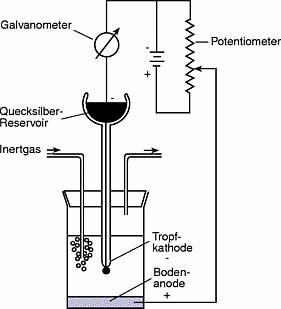
\includegraphics[width=0.4\textwidth]{img/Polarograph}
	\caption{Schematische Darstellung eines Polarographen \cite{Brehm.2004}}
	\label{fig:schema_polarograph}
\end{figure}
\FloatBarrier
%Ende

Im Versuch wurde mittels des Analyseverfahrens der Polarographie, der Bleigehalt in einer unbekannten Wasserprobe bestimmt.

\section{Theorie}
\label{sec:theorie}

Grundlage für die Analyse der enthaltenen Metall-Ionen ist die aufgenommene Strom-Spannungs-Kurve des Polarographen. Aufgrund der spezifischen Halbstufenpotentiale von Metall-Ionen ändert sich bei unterschiedlichen Arbeitspotentialen die gemessene Stromstärke. Dieser Strom an der Arbeitselektrode erfolgt aufgrund der Reduktionsreaktion der Metall-Ionen und ist direkt proportional zur Konzentration des umgesetzten Stoffes. Der Strom im Zusammenhang mit diesem Massentransport der Ionen wird als \textsc{Faraday}schen Strom bezeichnet. Um eine ausreichende Leitfähigkeit und somit einen entsprechenden Ladungstransport in der Lösung garantieren zu können werden den untersuchten Proben oft Grundelektrolyten in Form von Salzen, Säuren oder Basen zugegeben.\linebreak
Aufgrund der spezifischen Halbstufenpotentiale lassen sich qualitative Ergebnisse dieses Verfahrens auswerten. Betrachtet man jedoch auch den Zusammenhang des Stromflusses bei einem bestimmten Arbeitspotential mit der Konzentration des umgesetzten Stoffes, so lassen sich ebenfalls quantitative Bewertungen äußern.\linebreak
Für diese Betrachtung ist jedoch eine Form der Kalibrierung notwendig, um die gemessenen Signale quantitativ auswerten zu können. Dies ist zum einen über einen externen oder internen Standard möglich, jedoch wurde sich aufgrund der geringen zu bestimmenden Konzentrationen in diesem Versuch für die Aufstockmethode alias Standardadditionsmethode entschieden. Möchte man einen internen oder exterenen Standard nutzen so sind in diesem Fall ebenfalls Kalibrierkurven mit linearem Zusammenhang mittels bekannter Referenz aufzustellen.\linebreak
Bei dieser Methode wird in diesem Versuch nach dem polarographischen Messen der unbehandelten Probe eine definierte Menge eines bekannten Standards zugegeben. Dieser Standard enthält dabei den zu bestimmenden Stoff in einer exakt bekannten Konzentration. Aus den gemessenen Datenpunkten lässt sich nun eine Geradengleichung bestimmen (siehe Abb. \ref{fig:standardaddition} und Gl. \ref{gl:1}).

\begin{flalign}
\label{gl:1}
Y &= \frac{\Delta y}{\Delta x}*X+yA
\end{flalign}

%Start
\begin{figure}[h!]
	\centering
	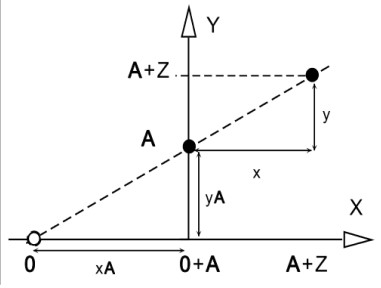
\includegraphics[width=0.5\textwidth]{img/Standardaddition}
	\caption{Darstellung der Standardadditionsmethode \cite{}}
	\label{fig:standardaddition}
\end{figure}
\FloatBarrier
%Ende

Aus der ermittelten Geradengleichung lässt sich nun aufgrund des geometrischen Beziehung des Strahlensatzes lässt sich die Konzentration der Probe über den Wert $x_A$ in Abb. \ref{fig:standardaddition} bestimmen. Eine Herleitung dazu in unter Gl. \ref{gl:2} und Gl. \ref{gl:3} zu finden.

\begin{flalign}
\label{gl:2}
	Y &= \frac{y}{x}*X+yA\\
	X&= \frac{Y-yA}{\frac{y}{x}}
\end{flalign}

\textit{Für $Y=0$ heißt das:}

\begin{flalign}
\label{gl:3}
X&= x_A = \frac{0-yA}{\frac{y}{x}} = \frac{-yA}{\frac{y}{x}}\\
x_A&= -c\\
c	&= \underline{\underline{\frac{yA}{\frac{y}{x}}}}
\end{flalign}







\section{Durchführung}
\label{sec:durchfuerung}

Die Versuchsanlage besteht aus mehreren, einzeln absperrbaren Rohrleitungen unterschiedlicher Durchmesser und teils mit Einbauten. Für den Versuch werden je drei Rohrleitungen – eine angeraute Leitung und zwei hydraulisch glatte Leitungen unterschiedlicher Nenndurchmesser – ohne Einbauten sowie je eine Rohrleitung mit eingebautem Schrägsitzventil und einem Muffenschieber untersucht. \\
Für die rauen und hydraulisch glatten Rohrleitungen werden dazu für je fünf unterschiedliche Wasservolumenströme die Druckverluste in jeder einzelnen Rohrleitung über die Manometer am Ein- und Auslauf ermittelt. \linebreak 
Vorher ist das System zu entlüften. Mittels der Druckverluste und der Strömungsgeschwindigkeiten berechnet sich schließlich für jede Rohrleitung eine entsprechende Rohrreibungszahl $\lambda$. \\
Die Rohrleitungen mit Einbauten werden auf die Druckverlustbeiwerte $\zeta$ untersucht, die durch die jeweiligen eingebauten Armaturen auftreten. Dazu werden die Druckverluste bei einem konstanten Wasservolumenstrom bestimmt, während die Öffnungsweite des Ventils bzw. des Muffenschiebers verändert wird. Die sich daraus ergebende Ventilkennlinie ist als $\zeta$ über den Öffnungswinkel und als kv-Wert über den Ventilhub aufzutragen. \\
Für die Rohrreibungszahl $\lambda$ ist zusätzlich eine Fehlerrechnung durchzuführen, da anzunehmen ist, dass die Messwerte des Versuchs mit Fehlern behaftet sind.\\
Neben der Versuchsanlage mit den Messinstrumenten für Druck und Volumenstrom wurde weiterhin eine Stoppuhr genutzt.

\chapter{Ergebnisse}
\label{sec:ergebnisse}



\section{Diskussion}
\label{sec:diskussion}


%Start
\begin{figure}[h!]
	\centering
	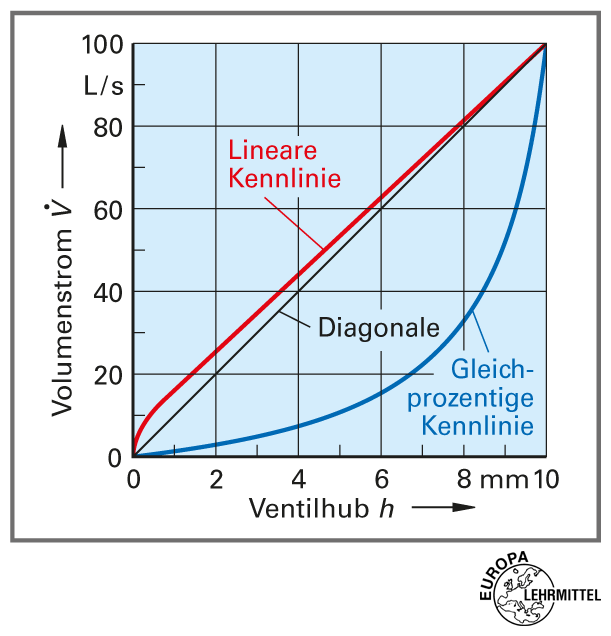
\includegraphics[width=0.5\textwidth]{img/035-3}
	\caption{Kennline von Ventilen \cite[S.35, Bild 3]{Ignatowitz.2013}}
	\label{fig:kennlinie_ct}
\end{figure}
\FloatBarrier
%Ende

\chapter{Fehlerbetrachtung}
\label{sec:fehler}

%Tabelle START
\vspace*{-2.5mm}
\renewcommand{\arraystretch}{1.2}
\begin{table}[h!]
	\centering
	\caption{Abweichungen für Fehlerrechnung}
	\label{tab:abweichungen}
	%\resizebox{10cm}{!}{
	\begin{tabulary}{\textwidth}{C|C}
		\hline 
		\textbf{Messgröße} & \textbf{Abweichung} \\ 
		\hline 
		Volumenstrom &  $\pm2,5\%$\\ 
		Temperatur & $\pm \SI{0.5}{\kelvin} $\\ 
		Druckmessungen &  $\pm \SI{2}{\milli \mws}$\\ 
		\hline 
	\end{tabulary}
	%}
\end{table}
\FloatBarrier
\vspace*{-2.5mm}
%Tabelle Ende


\chapter*{Anhang}
\addcontentsline{toc}{chapter}{Anhang}
\label{sec:anhang}

%Tabelle START
\vspace*{-2.5mm}
\renewcommand{\arraystretch}{1.2}
\begin{table}[h!]
	\centering
	\caption{Dichte des Wassers zu unterschiedlichen Temperaturen mittels \cite{BernhardSpang.2002}}
	\label{tab:dichte}
	%\resizebox{10cm}{!}{
	\begin{tabulary}{\textwidth}{C|C}
		\hline
		\textbf{Temperatur} & \textbf{Dichte mittels \texttt{=densW(T,p)}} \\ 
		\hline
		\SI{25,4}{\celsius} & \SI{996,98}{\kg\per\raiseto{3}\meter} \\
		\SI{25,5}{\celsius} & \SI{996,96}{\kg\per\raiseto{3}\meter} \\
		\SI{25,6}{\celsius} & \SI{996,93}{\kg\per\raiseto{3}\meter} \\
		\SI{25,7}{\celsius} & \SI{996,91}{\kg\per\raiseto{3}\meter} \\
		\SI{25,8}{\celsius} & \SI{996,88}{\kg\per\raiseto{3}\meter} \\
		\SI{25,9}{\celsius} & \SI{996,85}{\kg\per\raiseto{3}\meter} \\
		\SI{26,0}{\celsius} & \SI{996,83}{\kg\per\raiseto{3}\meter} \\
		\SI{26,1}{\celsius} & \SI{996,80}{\kg\per\raiseto{3}\meter} \\
		\SI{26,2}{\celsius} & \SI{996,77}{\kg\per\raiseto{3}\meter} \\
		\SI{26,3}{\celsius} & \SI{996,75}{\kg\per\raiseto{3}\meter} \\
		\SI{26,4}{\celsius} & \SI{996,72}{\kg\per\raiseto{3}\meter} \\
		\SI{26,5}{\celsius} & \SI{996,69}{\kg\per\raiseto{3}\meter} \\
		\SI{26,6}{\celsius} & \SI{996,67}{\kg\per\raiseto{3}\meter} \\
		\SI{26,7}{\celsius} & \SI{996,64}{\kg\per\raiseto{3}\meter} \\
		\SI{26,8}{\celsius} & \SI{996,61}{\kg\per\raiseto{3}\meter} \\
		\SI{26,9}{\celsius} & \SI{996,58}{\kg\per\raiseto{3}\meter} \\
		\SI{27,0}{\celsius} & \SI{996,56}{\kg\per\raiseto{3}\meter} \\
		\SI{27,1}{\celsius} & \SI{996,53}{\kg\per\raiseto{3}\meter} \\
		\SI{27,2}{\celsius} & \SI{996,50}{\kg\per\raiseto{3}\meter} \\
		\SI{27,3}{\celsius} & \SI{996,48}{\kg\per\raiseto{3}\meter} \\
		\SI{27,4}{\celsius} & \SI{996,45}{\kg\per\raiseto{3}\meter} \\
		\SI{27,5}{\celsius} & \SI{996,42}{\kg\per\raiseto{3}\meter} \\
		\hline
	\end{tabulary}
	%}
\end{table}
\FloatBarrier
\vspace*{-2.5mm}
%Tabelle Ende

%Praktikumsskript, Modul ………, Versuch …….., Prof. Musterprof. 
%DIN 12345, Jahr der Veröffentlichung 
%Link der Internetseite, Zugriffsdatum 
%Buchtitel, Autor, Verlag, Veröffentlichungsjahr 

%Literaturverzeichnis Bücher
\bibliography{Literatur}
\bibliographystyle{unsrtdin}
\addcontentsline{toc}{section}{Literaturverzeichnis}



%\chapter*{Eidesstattliche Erklärung}
\label{erklaerung}
Hiermit versichere ich, die vorliegende Seminararbeit selbstständig und nur unter Verwendung der von mir angegebenen Quellen und Hilfsmittel verfasst zu haben. Sowohl inhaltlich als auch wörtlich entnommene Inhalte wurden als solche kenntlich gemacht. Die Arbeit hat in dieser oder vergleichbarer Form noch keinem anderem Prüfungsgremium vorgelegen. \\
\\[1.5cm]
Datum:	\hrulefill\enspace Unterschrift: \hrulefill
\\[3.5cm]
\addcontentsline{toc}{chapter}{Selbstständigkeitserklärung}

%\chapter{Bausteine}

\section{Beispiel für Tabelle}

%Tabelle START
\vspace*{-2.5mm}
\renewcommand{\arraystretch}{1.2}
\begin{table}[h!]
	\centering
	\caption{Abmessungen der Probekörper vor dem Zugversuch}
	\label{tab:tabelle1}
	%\resizebox{10cm}{!}{
	\begin{tabulary}{\textwidth}{C|CCC}
		\hline
		\textbf{Probe}  &\textbf{Breite [mm]}&\textbf{Dicke [mm]}&\textbf{Anf.-länge[mm]} \\ 
		\hline
		Kupfer (gewalzt) & 12,5 &3,00&50\\
		Kupfer (geglüht) & 12,5&3,00&50\\
		PA6 & 10,0&4,00&50\\
		PP (EPR-30\% Kautschuk) & 9,9 &3,95&50\\
		\hline
	\end{tabulary}
	%}
\end{table}

\FloatBarrier
\vspace*{-2.5mm}
%Tabelle ENDE

\section*{Tabelle mit Itemize}
%Tabelle START
\vspace*{-2.5mm}
\renewcommand{\arraystretch}{1.2}
\begin{table}[h!]
	\centering
	\caption*{Vor- und Nachteile der Geothermie}
	\label{tab:tabelle1}
	\begin{tabulary}{\textwidth}{C|C}
		\hline
		\textbf{Vorteile}  &\textbf{Nachteile} \\ 
		\hline
		&\\
		\begin{minipage}[t]{0.4\textwidth}
			\begin{itemize}
				\item Strom, Wärme und Kälte wird erzeugt
				\item keine saisonalen und tageszeitlichen Schwankungen
				\item 	quasi-regenerativ
				\item 	nachfrage-gerechte Energiebereitstellung
				\item Erzeugungspotenzial sehr hoch 
				\item 	grundsätzlich standortunabhängig
			\end{itemize}
		\end{minipage} & 
		\begin{minipage}[t]{0.4\textwidth}
			\begin{itemize}
				\item hohe Anschaffungskosten
				\item abhängig von geologischen Gegebenheiten
				\item geringer Stromwirkungsgrad (thermodynamisch bedingt)
				\item keine Marktdurchdringung in DE
				\item erfahrene Bauunternehmen notwendig
				\item gute Vorerkundung und Überwachung notwendig
			\end{itemize}
		\end{minipage}\\
	\end{tabulary}
\end{table}
\FloatBarrier
\vspace*{-2.5mm}
%Tabelle ENDE

\newpage

\section*{Beispiel für Skalierbare Tabelle}
%TAbelle Start
\vspace*{-2.5mm}
\renewcommand{\arraystretch}{1.2}
\begin{table}[h!]
	\centering
	\caption*{}
	\resizebox{0.5\textwidth}{!}{
		\begin{tabulary}{\textwidth}{C|C|C|C}
			\textbf{Name} & \textbf{Anwendung}&\textbf{Gleichung}&\textbf{Stoffkonstante} \\ 
			\hline  
			KICK& $x_{80_\omega}>\SI{50}{\milli\meter}$ &$e_{KICK}=c_K*log(\frac{x_{80_\omega}}{x_{80_\alpha}})$&$c_K=1,15*\frac{c_B}{\sqrt{0,05\si{\meter}}} \left[\si{\raiseto{2}\meter\per\raiseto{2}\second}\right]$\\
			BOND&$\SI{50}{\micro\meter}<x_{80_\omega}<\SI{50}{\milli\meter}$&$e_{BOND}=c_B*\left(\frac{1}{\sqrt{x_{80_\omega}}}-\frac{1}{\sqrt{x_{80_\alpha}}}\right)$& $c_B$: tabelliert $\left[\si{\raiseto{2,5}\meter\per\raiseto{2}\second}\right]$\\ 
			RITTER& $x_{80_\omega}>\SI{50}{\micro\meter}$&$e_{RITT}=c_R*\left(\frac{1}{x_{80_\omega}}-\frac{1}{x_{80_\alpha}}\right)$&$c_R= 0,5*c_B*\sqrt{\SI{5e-5}{\meter}}$ \\  
	\end{tabulary}}
\end{table}
\FloatBarrier
%Ende TAbelle

\section{Befehlszeilen in Text einfügen}
Befehlzeilen aus der "Latex-Sprache"\ lassen sich nicht ohne weiteres im Text darstellen. Das System erkennt diese als solche und gibt warnhinweise aus. In der Regel werden die Befehle dann auch falsch dargestellt. Umgehen lässt sich diese Problematik mit der verbatim-Umgebung. In ihren Grenzen werden Eingaben 1:1 dargestellt wie eingegeben. Die Funktionsweise soll nachfolgend durch ein Beispiel verdeutlicht werden.
\begin{verbatim*}

\begin{verbatim}
\usepackage{Beispieltrolllllollllolll} 
\end{verbatim}

\end{verbatim*}

Sollte besonderer Wert auf die Kenntlichmachung der Leerzeichen gelegt werden kann auch mit \texttt{verbatim*} gearbeitet werden.

\section{Seitenübergreifende, lange Tabellen}

Tabellen welche Messwerte in einem solchen Umfang enthalten, dass sie nicht auf einer einzelnen A4-Seite Platz finden, können mit dem Paket \begin{verbatim}
\usepackage{longtable} 
\end{verbatim}
in ein Dokument eingepflegt werden wie folgendes Beispiel belegt.:
\begin{longtable}[c]{lllll}
	\caption{Dehnungstabelle}\\
	\label{alles}
	$Zeit [HH:MM:SS]$ & $\Delta l_{PE} [mm]$ & $\varepsilon_{PE}$ & $\Delta l_{Pb} [mm]$ & $\varepsilon_{Pb}$ \\
	\hline
	\endfirsthead
	%\caption{}\\
	$Zeit [HH:MM:SS]$ & $\Delta l_{PE} [mm]$ & $\varepsilon_{PE}$ & $\Delta l_{Pb} [mm]$ & $\varepsilon_{Pb}$ \\ 
	\hline
	\endhead
	\multicolumn{5}{r}{Fortsetzung auf n{\"a}chster Seite}\\
	\endfoot
	\hline
	\multicolumn{5}{r}{} \\
	\endlastfoot
	% Ab hier kommt der Inhalt der Tabelle
	00:00:00 & 3,00 & 0,11 & 3,30 & 0,12\\
	00:00:10 & 3,80 & 0,14 & 3,42 & 0,13\\
	00:00:20 & 4,15 & 0,16 & 3,53 & 0,13\\
	00:00:30 & 4,43 & 0,17 & 3,68 & 0,14\\
	00:00:40 & 4,61 & 0,17 & 3,71 & 0,14\\
	00:00:50 & 4,80 & 0,18 & 3,81 & 0,14\\
	00:01:00 & 4,95 & 0,19 & 4,12 & 0,15\\
	00:20:00 & 8,03 & 0,30 &  & \\
\end{longtable} 

\section{Diagramme}
Diagramme lassen sich unter anderem mit dem Paket 
\begin{verbatim}
\usepackage{pgfplots} 
\end{verbatim}
implementieren.
Um das Dokument einigermaßen klein zu halten empfehle ich folgendes weiters Paket zu nutzen.
\begin{verbatim}
\usepackage{csvsimple} 
\end{verbatim}
Es erleichter das importieren von Datensätzen aus .csv Dateien. Die .csv Datei muss folgenden Anforderungen genügen:- Dezimaltrenner Punkt
\begin{itemize}
	\item Dezimaltrenner Punkt
	\item Jede Zeile umgebrochen
	\item Koordinaten durch komma getrennt
	\item Spalten beschriften z.B x,y oder a,b
\end{itemize}

Sollte man eine Tabellenkalkulationsdatei in eine csv Datei konvertiert haben, hat dieses meist die Falsche Form. Durch die Funktion suchen und ersetzen (bsp emacs) können aber sehr schnell die nötigen Korrekturen erfolgen. 

\begin{figure}[h]
	\begin{center}
		\begin{tikzpicture}
		\begin{axis}[
		width=12cm,
		height=6cm,
		xlabel=Zeit in Sekunden,
		ylabel=Dehnung]
		
		\begin{scope}[brown]
		\draw[brown] ({axis cs:10,0}|-{rel axis cs:0,1}) -- ({axis cs:10,0}|-{rel axis cs:0,0});
		\draw[brown] ({axis cs:120,0}|-{rel axis cs:0,1}) -- ({axis cs:120,0}|-{rel axis cs:0,0});
		\end{scope} 
		
		\addplot table [x=a, y=b, col sep=comma] {data/KriechkurvePb.csv};
		\end{axis}
		\end{tikzpicture}
		\caption{Kriechkurve Blei}
		\label{kkb}
	\end{center}
\end{figure} 
\FloatBarrier                     

\section*{Beispiel für Berechnungen}
Die Berechnung der wahren Spannung $\sigma_{W}$ bei Höchstkraft erfolgt unter der Annahme, dass der Prüfkörperquerschnitt noch 60\% des Ausgangsquerschnitts beträgt. Die Berechnung erfolgt ab Gleichung \ref{ber1}.\\ 

%Berechnung der Fläche A
\textbf{Fläche} $\boldsymbol{A}$ \textbf{:}
%Start
\begin{flalign}
A 	&= \frac{\pi}{4}*d^2\\
&=\frac{\pi}{4}*(\SI{80}{\milli \meter})^2
\end{flalign}
%Ende

\section{Beispiel für ein Bild}

%Start
\begin{figure}[h!]
	\centering
	\includegraphics[width=0.60\textwidth]{img/skizzepruef3}
	\caption{Skizze Prüfkörperbemaßung}
	\label{skizzepruef}
\end{figure}
\FloatBarrier
%Ende

\newpage

\section{Beispiel für zwei Bilder}
\label{sec:versuchsaufbau}

%Start
\begin{figure}[h!]
	\centering
	\begin{subfigure}{.5\textwidth}
		\centering
		\includegraphics[width=0.75\textwidth]{Aufbau2}
		\caption{Skizze zum Versuchsaufbau}
		\label{fig:sub1}
	\end{subfigure}%
	\begin{subfigure}{.5\textwidth}
		\centering
		\includegraphics[width=0.6\textwidth]{img/Aufbau1}
		\caption{realer Versuchsaufbau}
		\label{fig:sub2}
	\end{subfigure}
	\caption{Versuchsaufbau als Skizze und in Realität}
	\label{fig:aufbau} 
\end{figure}
\FloatBarrier
%Ende

\newpage


\section{Beispiel für vier Bilder}
%Start
\begin{figure}[h!]
	\centering
	\begin{subfigure}{.5\textwidth}
		\centering
		\includegraphics[width=0.75\textwidth]{img/Kupfer_gewalzt}
		\caption{Kupfer (gewalzt)}
		\label{fig:sub3}
	\end{subfigure}%
	\begin{subfigure}{.5\textwidth}
		\centering
		\includegraphics[width=0.75\textwidth]{img/Kupfer_weich}
		\caption{Kupfer (geglüht)}
		\label{fig:sub4}
	\end{subfigure}
	\begin{subfigure}{.5\textwidth}
		\centering
		\includegraphics[width=0.75\textwidth]{img/PA6}
		\caption{PA6}
		\label{fig:sub5}
	\end{subfigure}%
	\begin{subfigure}{.5\textwidth}
		\centering
		\includegraphics[width=0.75\textwidth]{img/PP}
		\caption{PP (ERP-30\% Kautschuk)}
		\label{fig:sub6}
	\end{subfigure}
	
	\caption{Bruchstellennahaufnahmen der Probekörper}
	\label{fig:bruchstellen} 
\end{figure}
\FloatBarrier
%Ende

\section{Beispiel Einheiten}

\begin{align*}
\textbf{$\SI{12,0/12}{\kg\meter\per\second \raiseto{5} \per \xyz}*\SI{13}{\per\raiseto{-2}\meter}=\SI{256}{}$}
\end{align*}

\begin{align}
\SI{12,0/12}{\meter\per\joule}*\SI{13}{\gram}=\SI{256}{\coulomb}
\end{align}

\newpage

\section{Beispiel für Mini-Formelsammlung}
\begin{flalign}
\label{gl1}
\text{\textbf{Dehnung (Def.)} } \boldsymbol{\varepsilon} \text{ \textbf{:}} && \hspace*{-1em}  \varepsilon=\frac{\Delta l}{l_0} &&
\end{flalign}

\begin{flalign}
\label{gl2}
\text{\textbf{norminelle Spannung} } \boldsymbol{\sigma} \text{\textbf{:}} && \hspace*{-3em} \sigma=\frac{F}{A_0} &&
\end{flalign}

\begin{flalign}
\label{gl3}
\text{\textbf{Sekantenmodul (Kunststoffe) }} \boldsymbol{E_S} \text{ \textbf{:}} && E_S=\frac{\sigma_2-\sigma_1}{\varepsilon_2-\varepsilon_1}=\frac{F_2-F_1}{0,002*A_0} &&
\end{flalign}

\begin{flalign}
\label{gl4}
\text{\textbf{E-Modul (Metalle) }} \boldsymbol{E_M} \text{ \textbf{:}} && \hspace*{5em} E_M=\frac{\sigma}{\varepsilon}=\frac{\sigma_2-\sigma_1}{\varepsilon_2-\varepsilon_1}=\frac{R_{p_{0.2\%}}}{0,2\%} &&
\end{flalign}

\begin{flalign}
\label{gl5}
\text{\textbf{Bruchdehnung} } \boldsymbol{A} \text{\textbf{:}} && \hspace*{6em} A= \frac{l_{u}-l_{0}}{l_{0}}*100\% &&
\end{flalign}

\begin{flalign}
\label{gl6}
\text{\textbf{Ausgangsquerschnitt } } \boldsymbol{S_0} \text{\textbf{:}} && \hspace*{3em} S_{0}= Breite*Dicke &&
\end{flalign}
\begin{flalign}
\label{gl7}
\text{\textbf{wahre Spannung} } \boldsymbol{\sigma_{W}} \text{\textbf{:}} &&\hspace*{1em} \sigma_{W}=\frac{F_{max}}{S_{End}}&&
\end{flalign}
\begin{flalign}
\label{gl8}
\text{\textbf{Brucheinschnürung } } \boldsymbol{Z} \text{\textbf{:}} && \hspace*{5em} Z=\frac{S_0-S_u}{S_{o}}*100\% &&
\end{flalign}

\newpage

\section*{Fußnoten}
%Start
\begin{figure}[h!]
	\centering
	\includegraphics[width=0.85\textwidth]{tabdia/kfwerte}
	\caption*{$\text{k}_\text{f}$-Werte der Proben 1 bis 11 \protect\footnotemark[1]}
	\label{}
\end{figure}
\FloatBarrier
%Ende

\footnotetext[1]{bezogen auf $V=\SI{50}{\milli \liter}$ und $h=\SI{10}{\milli \meter}$}



\end{document}
